In this section, the results obtained will be shown and compared. Each solution was tested on the proposed graphs in \ref{sec:graph} to verify their behavior in different contexts. 
The test has been executed on \textbf{Xeon PHI}, with $64$ cores and $4$ hardware thread per core. 

\subsection{Real Results}
In the table (\ref{table:seq_times}) below, are included the sequential times used in the plots and to compute the speedup of the various solutions.
\begin{table}[htb!]
\centering
\begin{tabular}{|c|c|c|c|}
\hline
Sequential & 10K 0.02D & 10K 0.5D & 10K 0.8D \\ \hline
Time ($\mu sec$)          & 21964     & 162399   & 359583   \\ \hline
\end{tabular}
\caption{Time results of the sequential executions.}
\label{table:seq_times}
\end{table}
\FloatBarrier

The following plots show the performance trend of the proposed solutions, starting from the low dense graph. The tests of the dynamic scheduling version were performed with chunk size of $32$, $64$ and $128$. 

In this first graph, with density equal to $0.02$, all the four solution have the same behavior also for the performance drop around the $10$ workers. Moreover, the dynamic solution with chunk size of $128$ the knee point comes before due the smaller size of the frontiers.
\begin{figure}[htb!]
    \centering
    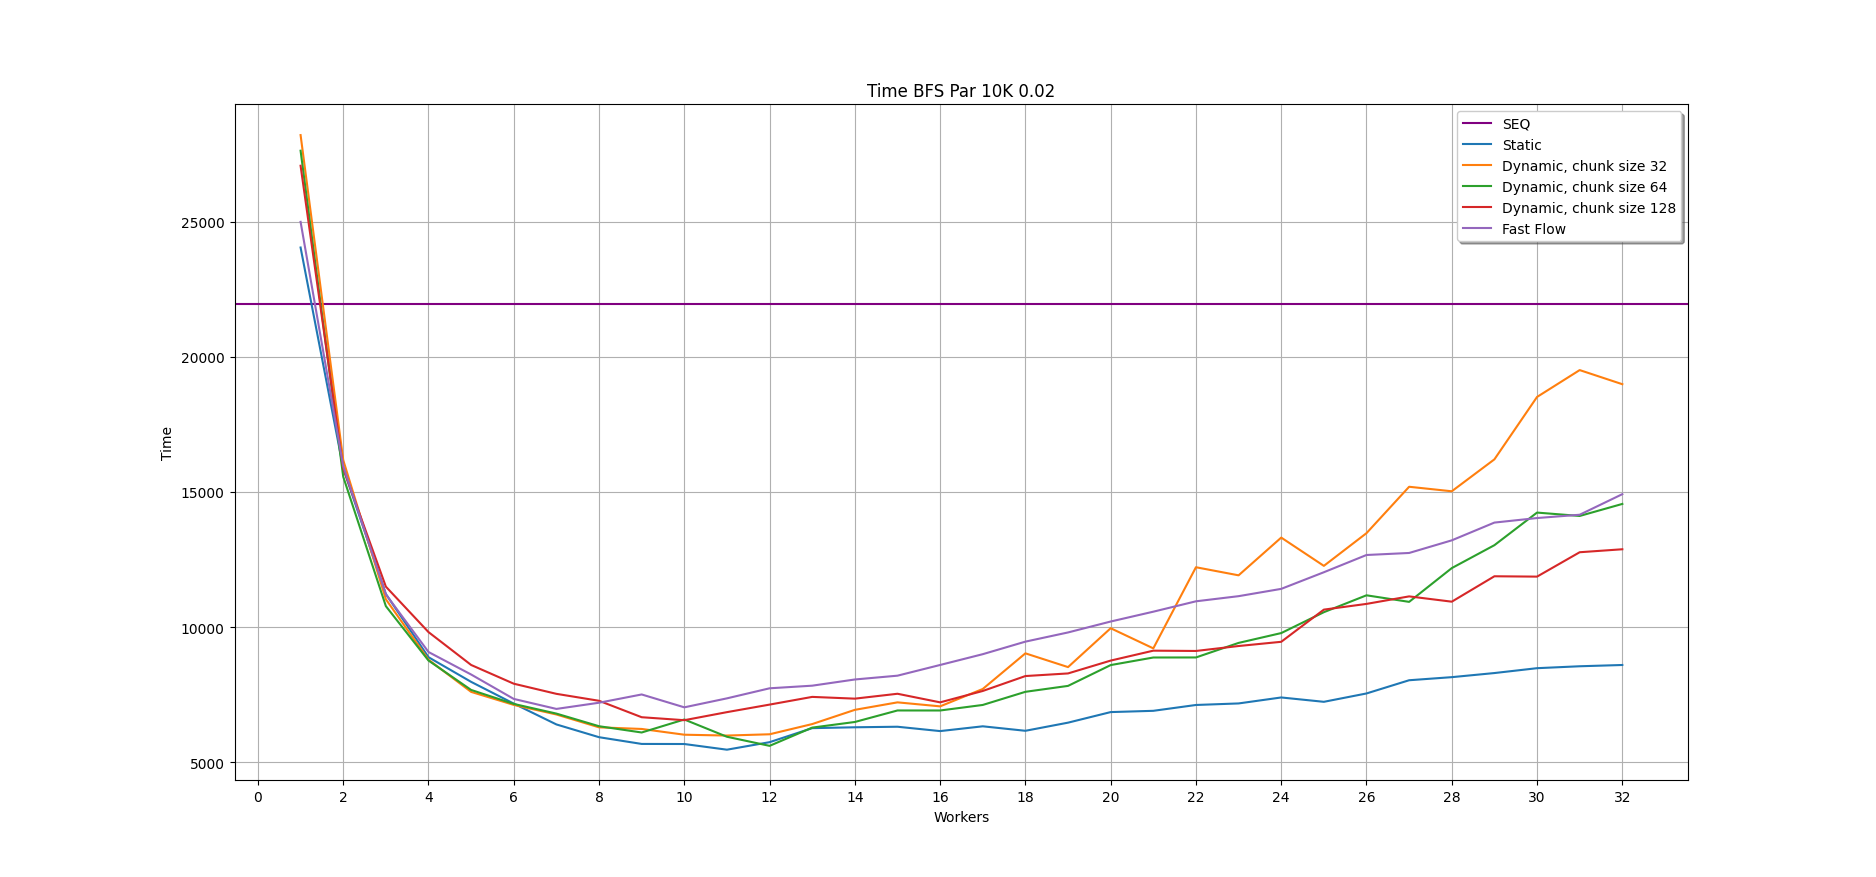
\includegraphics[width=\textwidth]{Figures/plot_map_time_vs10K002.png}
    \caption{Time plot graph 0.02 density.}
    \label{fig:plot_time_10k_002}
\end{figure}
\FloatBarrier

\begin{figure}[htb!]
    \centering
    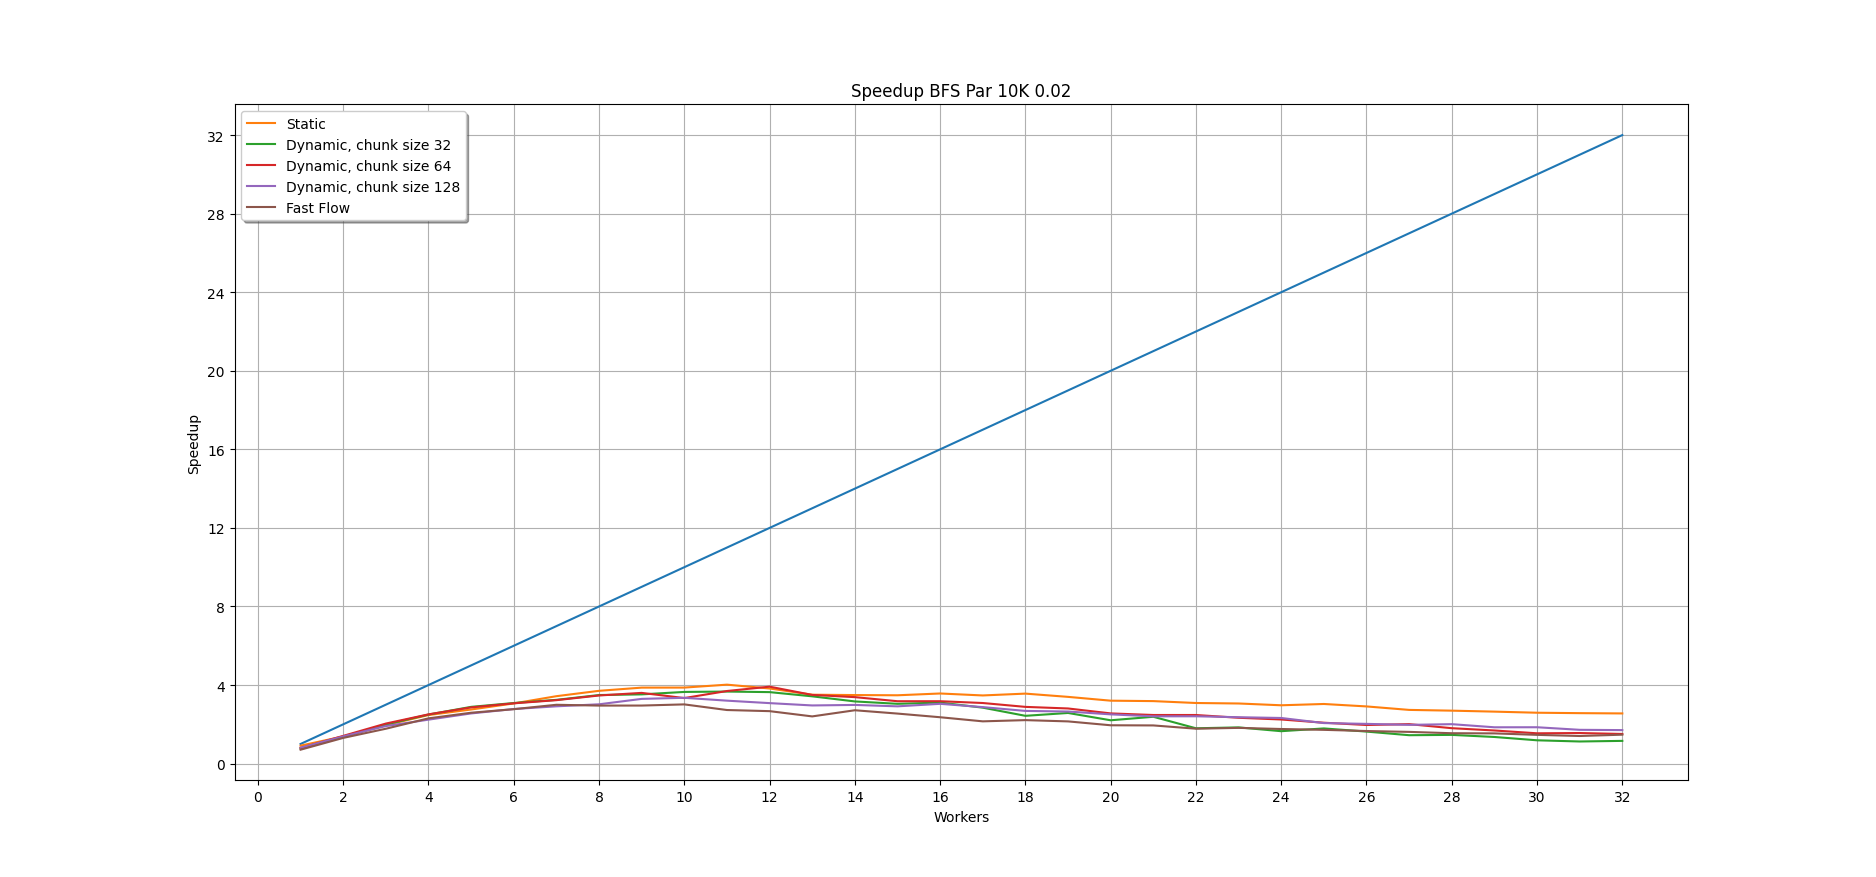
\includegraphics[width=\textwidth]{Figures/plot_map_speedup_vs10K002.png}
    \caption{Speedup plot graph 0.02 density.}
    \label{fig:plot_speedup_10k_002}
\end{figure}
\FloatBarrier
Growing density to $0.5$, and so the frontier size, the static version starts to suffer of load balancing problems mainly in with lower $nw$. Indeed, static approaches, the speedup growth is limited by the large size of the chunks that give the possibility to the first workers to visit most of the graph nodes creating a bottleneck. Meanwhile, dividing the frontier in smaller chunks provides the possibility to handle efficiently the free workers. In fact, the dynamic verison performance are better, in particular for the version with chunk of $32$ nodes.

\begin{figure}[htb!]
    \centering
    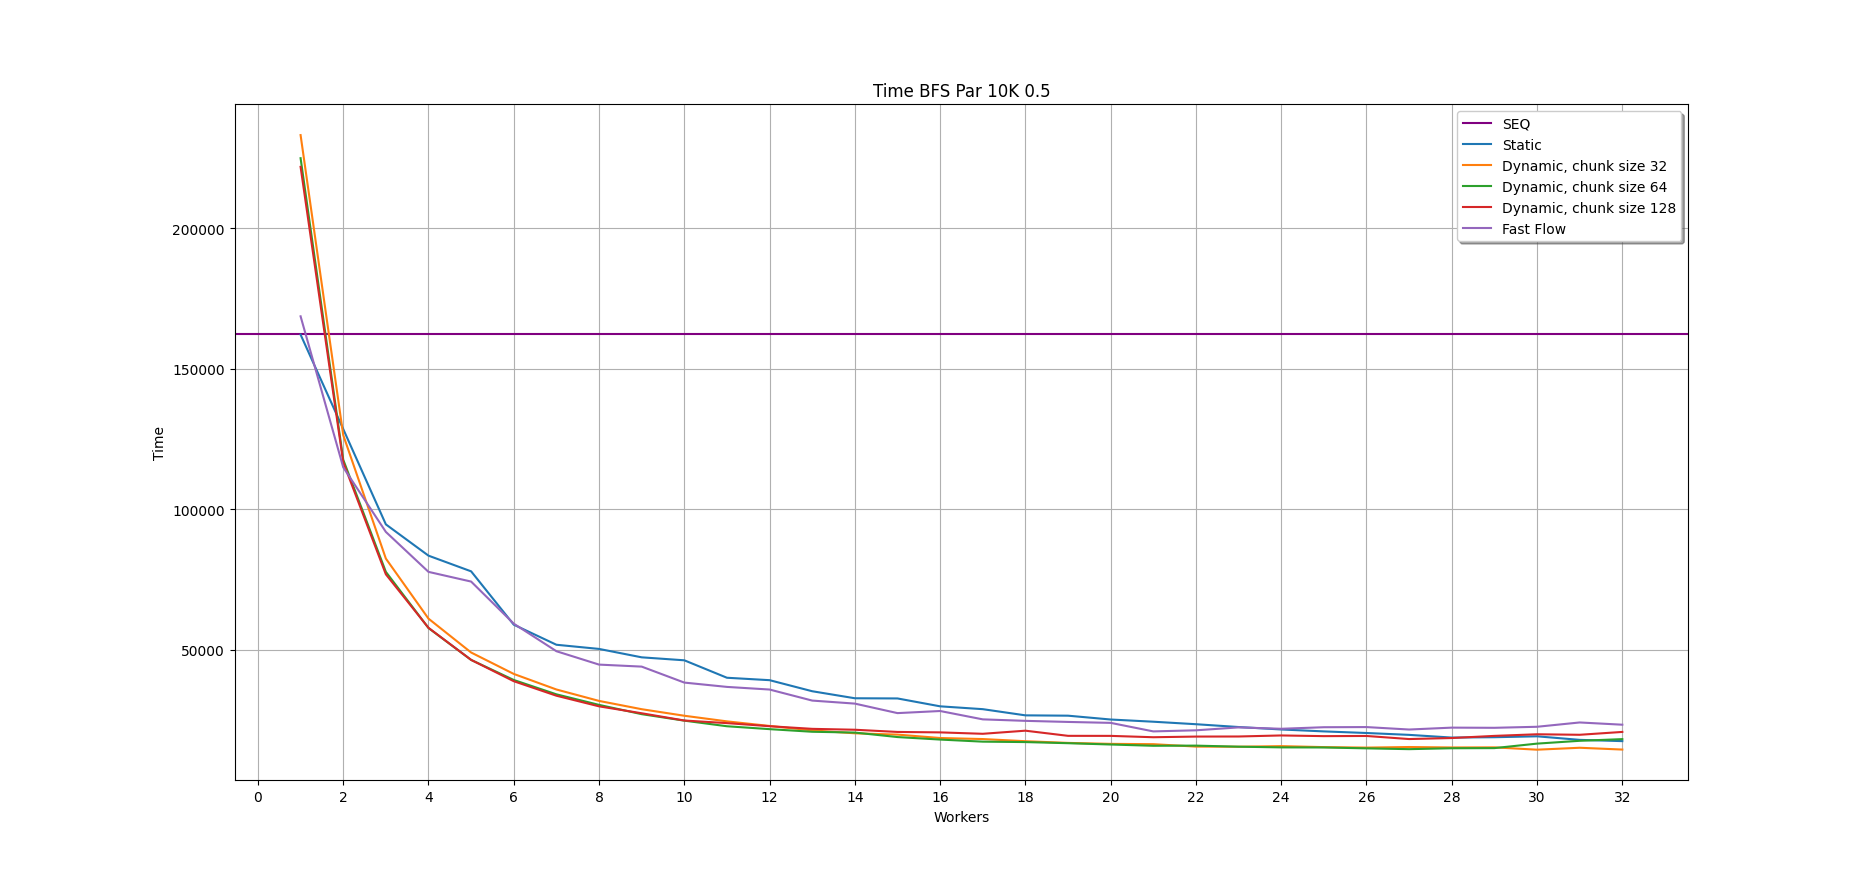
\includegraphics[width=\textwidth]{Figures/plot_map_time_vs10K05.png}
    \caption{Time plot graph 0.5 density.}
    \label{fig:plot_time_10k_05}
\end{figure}
\FloatBarrier

\begin{figure}[htb!]
    \centering
    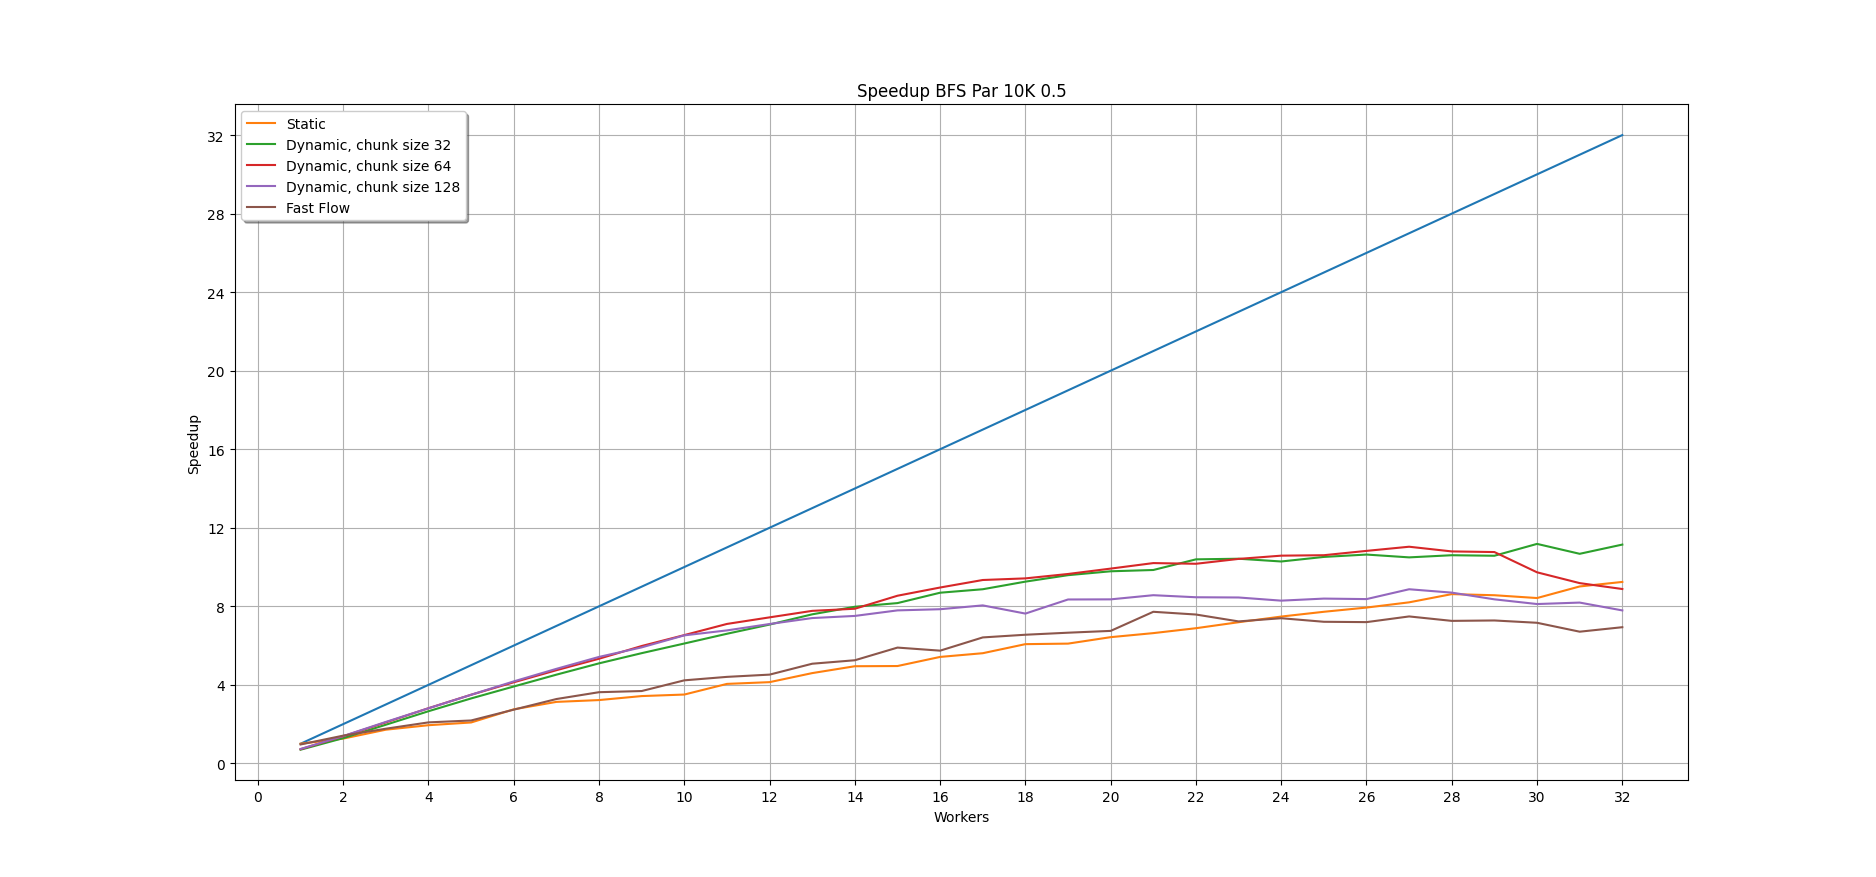
\includegraphics[width=\textwidth]{Figures/plot_map_speedup_vs10K05.png}
    \caption{Speedup plot graph 0.5 density.}
    \label{fig:plot_speedup_10k_05}
\end{figure}
\FloatBarrier

The analysis of the last graph shows, also in this case, better results for dynamic scheduling. In general, it is possible to see an improvement in performance by all solutions, this is due to the size of the frontiers that give the possibility to show the true potential of parallelization. From further tests performed, on this and other more populated and denser graphs, it was seen that the static scheduling versions achieve remarkable speedups but with a much higher number of threads than the dynamic version. In light of this it is necessary to make a consideration, the trend of the speedup (\ref{fig:plot_speedup_10k_08}) of the dynamic versions, compared to the static ones, shows very \textbf{high efficiency} and therefore ensuring a better trade-off for the cost-benefit aspect and so optimizing the usage of the provided hardware.

\begin{figure}[htb!]
    \centering
    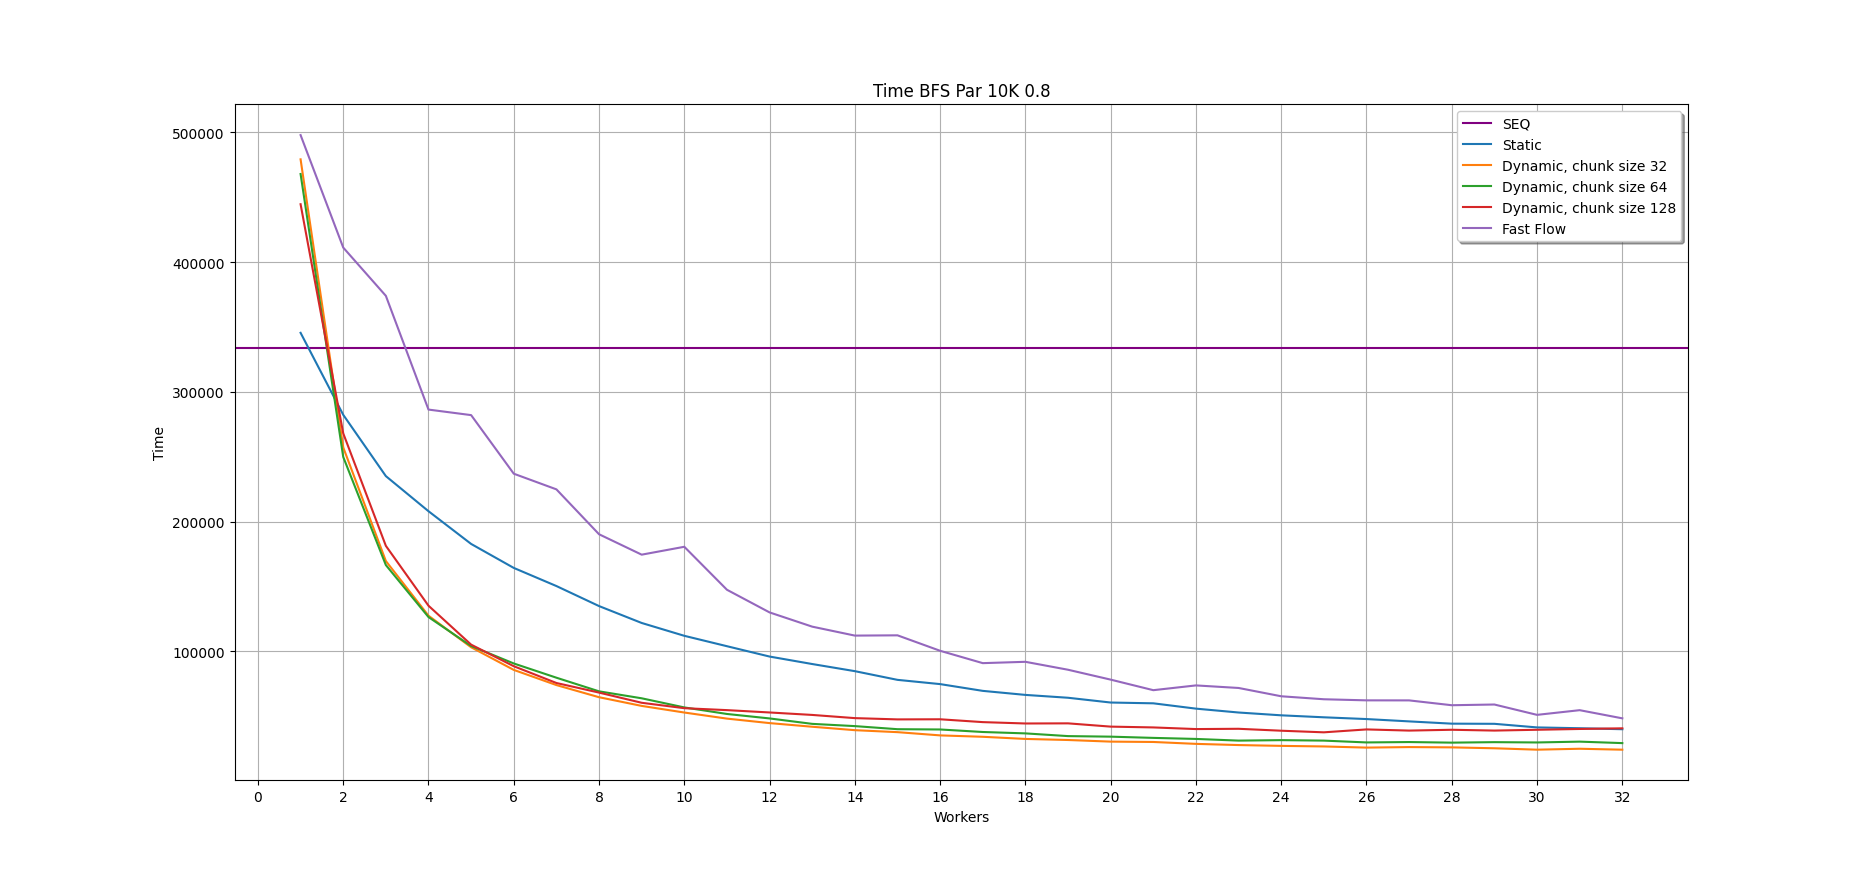
\includegraphics[width=\textwidth]{Figures/plot_map_time_vs10K08.png}
    \caption{Time plot graph 0.8 density.}
    \label{fig:plot_time_10k_08}
\end{figure}
\FloatBarrier

\begin{figure}[htb!]
    \centering
    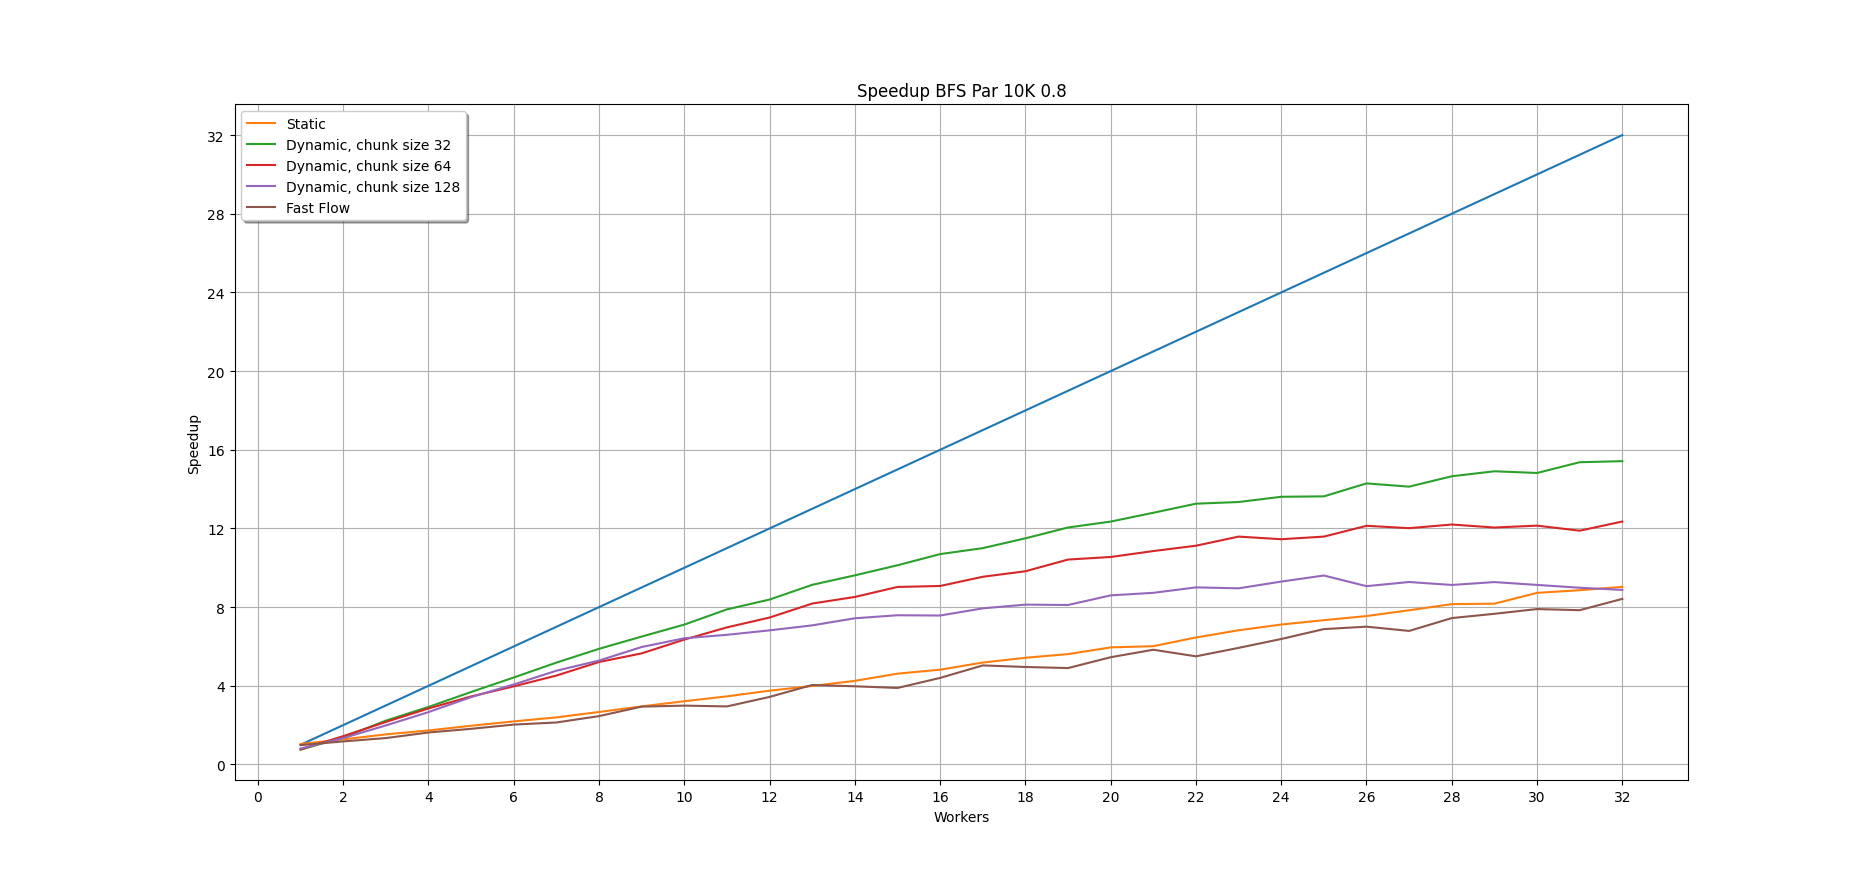
\includegraphics[width=\textwidth]{Figures/plot_map_speedup_vs10K08.png}
    \caption{Speedup plot graph 0.8 density.}
    \label{fig:plot_speedup_10k_08}
\end{figure}
\FloatBarrier

In the following tables you can see the speedup trend from a numerical point of view for all versions.

\begin{table}[!htb]
    \centering
    \begin{minipage}{0.08\textwidth}
    \centering
    \begin{tabular}{|c|}
    \hline
    NW \\ \hline
    1          \\ \hline
    2      \\ \hline
    4           \\ \hline
    8            \\ \hline
    16       \\ \hline
    32          \\ \hline
    \end{tabular}
    \end{minipage}
    \begin{minipage}{0.43\textwidth}
    \centering
    \begin{tabular}{|c|c|c|}
    \hline
    10K 0.02D & 10K 0.5D & 10K 0.8D \\ \hline
    0,913606  & 1,001233 & 1,040779 \\ \hline
    1,383123  & 1,262705 & 1,273857 \\ \hline
    2,471753  & 1,943502 & 1,729321 \\ \hline
    3,705753  & 3,223546 & 2,667787 \\ \hline
    3,569641  & 5,421432 & 4,819437 \\ \hline
    2,554548  & 9,240867 & 9,029531 \\ \hline
    \end{tabular}
    \end{minipage}
    \begin{minipage}{0.43\textwidth}
    \centering
    \begin{tabular}{|c|c|c|}
    \hline
    10K 0.02D & 10K 0.5D & 10K 0.8D \\ \hline
    0,878912  & 0,962564 & 0,981866 \\ \hline
    1,376535  & 1,412079 & 1,171711 \\ \hline
    2,419209  & 2,087579 & 1,625403 \\ \hline
    3,049708  & 3,624897 & 2,45788  \\ \hline
    2,55425   & 5,740509 & 4,400507 \\ \hline
    1,472414  & 6,93509  & 8,418585 \\ \hline
    \end{tabular}
    \end{minipage}
    \caption{Speedup phtread static scheduling (left) and Fast Flow solution (right).}
    \label{table:spup_static}
    \end{table}
\FloatBarrier

\begin{table}[htb!]
\centering
\begin{tabular}{|c|c|c|c|}
\hline
Workers & 10K 0.02D & 10K 0.5D & 10K 0.8D \\ \hline
1       & 0,778865  & 0,696421 & 0,750639 \\ \hline
2       & 1,357478  & 1,284081 & 1,378061 \\ \hline
4       & 2,497896  & 2,655661 & 2,922916 \\ \hline
8       & 3,490782  & 5,093752 & 5,879286 \\ \hline
16      & 3,107527  & 8,691875 & 10,69519 \\ \hline
32      & 1,156913  & 11,14306 & 15,42083 \\ \hline
\end{tabular}
\caption{Speedup dynamic scheduling solution with chunk size of 32 nodes.}
\label{table:spup_dy}
\end{table}
\FloatBarrier